\documentclass[fleqn]{article}
\usepackage[spanish]{babel}
\usepackage{amsmath}
\usepackage{amsthm}
\usepackage{graphicx}
\usepackage[utf8]{inputenc}

%%%%%%%% MARGIN
\usepackage[left=1in, right=1in, top=0.8in, bottom=0.8in]{geometry}

%%%%%%%% NO PARAGRAPH INDENT
% https://tex.stackexchange.com/questions/27802/set-noindent-for-entire-file
\setlength\parindent{0pt}

%%%%%%%% SUB-FIGURE PACKAGE
\usepackage{subcaption}

%%%%%%%% HYPERREF PACKAGE
\usepackage{hyperref}
\hypersetup{linkcolor=blue}
\hypersetup{citecolor=blue}
\hypersetup{urlcolor=blue}
\hypersetup{colorlinks=true}

%%%%%%%% MULTI-COLUMNS PACKAGE
\usepackage{multicol}

%%%%%%%% SETS DEFINITIONS
\usepackage{amssymb}
%%%% Important sets
\renewcommand{\O}{\mathbb{O}}
\newcommand{\N}{\mathbb{N}}
\newcommand{\Z}{{\mathbb{Z}}}
\newcommand{\Q}{{\mathbb{Q}}}
\newcommand{\R}{{\mathbb{R}}}

%%%% Statistics
\newcommand{\E}[1]{\mathbb{E}\left[#1 \right]}
\newcommand{\V}[1]{\mathrm{Var}\left[#1 \right]}

%%%% Lambda Calculus Symbols
\newcommand{\dneq}{\,\, \# \,\,}
\renewcommand{\S}{\pmb{\mathrm{S}}}
\newcommand{\I}{\pmb{\mathrm{I}}}
\newcommand{\K}{\pmb{\mathrm{K}}}
\newcommand{\ch}[1]{\ulcorner #1 \urcorner}

%%%% Ordinal Lambda Calculus Symbols
\newcommand{\ordAlph}{\Sigma_{\text{Ord}}}
\newcommand{\termOrd}{\text{Term}_\text{Ord}}
\newcommand{\fl}{\mathrm{fl}}
\newcommand{\sk}{\mathrm{sk}}

%%%% Superscript to the left
% https://latex.org/forum/viewtopic.php?t=455
\usepackage{tensor}
\newcommand{\app}[3]{\tensor*[^{#1}]{\left(#2, #3\right)}{}}

%%%% Make optional parameter
% https://tex.stackexchange.com/questions/217757/special-behavior-if-optional-argument-is-not-passed
\usepackage{xparse}
\NewDocumentCommand{\cx}{o}{
  \IfNoValueTF{#1}
  {\left[\quad\right]}
  {\left[\, #1 \,\right]}
}

%%%%%%%% LOGIC TREES
\usepackage{prftree}

%%%%%%%% SPLIT EQUATIONS
% https://tex.stackexchange.com/questions/51682/is-it-possible-to-pagebreak-aligned-equations
\allowdisplaybreaks

%%%%%%%% EXAM PACKAGE
\usepackage{mathexam}

%%%%%%%% CHANGE MARGINS ITEMIZE
\usepackage{enumitem}

\usepackage{float}

%%%%%%%% START DOCUMENT

\ExamClass{PROCESOS ESTOCÁSTICOS II}
\ExamName{TALLER TEÓRICO}
\ExamHead{\today}

\let\ds\displaystyle

\begin{document}
 \vspace{0.3cm}
   % Information of the student
   \begin{itemize}[leftmargin=6.25cm, labelsep=0.5cm]

     \item[\textit{Nombre}] \scalebox{1.2}{Juan Sebastián Cárdenas Rodríguez} % Name
     \item[\textit{Código}] 201710008101 % Code

   \end{itemize}
\vspace{0.3cm}

% Each of the items to solve
\begin{enumerate}
\item Pregunta 1.
  \begin{itemize}
  \item Ecuación 1
    \begin{enumerate}[label=\alph*)]
    \item Solución:
      \begin{figure}[H]
        \centering
        \includegraphics[scale=0.7]{exerc/11a}
      \end{figure}
    \item Solution
      \begin{figure}[H]
        \centering
        \includegraphics[scale=0.7]{exerc/11b}
        \caption{Primera parte.}
      \end{figure}
      \begin{figure}[H]
        \centering
        \includegraphics[scale=0.7]{exerc/11b2}
        \caption{Segunda parte.}
      \end{figure}
    \item Solución:
      \begin{figure}[H]
        \centering
        \includegraphics[scale=0.7]{exerc/11c}
      \end{figure}
    \item Solución:
      \begin{figure}[H]
        \centering
        \includegraphics[scale=0.7]{exerc/11d}
      \end{figure}
    \end{enumerate}
  \item Ecuación 2.
    \begin{enumerate}[label=\alph*)]
    \item Solución:
      \begin{figure}[H]
        \centering
        \includegraphics[scale=.7]{exerc/12a}
        \caption{Primera parte.}
      \end{figure}
      \begin{figure}[H]
        \centering
        \includegraphics[scale=.7]{exerc/12a2}
        \caption{Segunda parte.}
      \end{figure}
    \item Solución:
      \begin{figure}[H]
        \centering
        \includegraphics[scale=.7]{exerc/12b}
        \caption{Primera parte.}
      \end{figure}
      \begin{figure}[H]
        \centering
        \includegraphics[scale=.7]{exerc/12b2}
        \caption{Segunda parte.}
      \end{figure}
    \item Solución:
      \begin{figure}[H]
        \centering
        \includegraphics[scale=.7]{exerc/12c}
      \end{figure}
    \item Solución:
      \begin{figure}[H]
        \centering
        \includegraphics[scale=.7]{exerc/12d}
      \end{figure}
    \end{enumerate}
  \item Ecuación 3.
    \begin{enumerate}[label=\alph*)]
    \item Solución:
      \begin{figure}[H]
        \centering
        \includegraphics[scale=.7]{exerc/13a}
      \end{figure}
    \item Solución:
      \begin{figure}[H]
        \centering
        \includegraphics[scale=.7]{exerc/13b}
      \end{figure}
    \item Solución:
      \begin{figure}[H]
        \centering
        \includegraphics[scale=.7]{exerc/13c}
      \end{figure}
    \item Solución:
      \begin{figure}[H]
        \centering
        \includegraphics[scale=.7]{exerc/13d}
      \end{figure}
    \end{enumerate}
  \end{itemize}

\item Pregunta 2.
  \begin{itemize}
  \item Ecuación 1.
    \begin{enumerate}[label=\alph*)]
    \item Solución.
      \begin{figure}[H]
        \centering
        \includegraphics[scale=.7]{exerc/21a}
      \end{figure}
    \item Solución.
      \begin{figure}[H]
        \centering
        \includegraphics[scale=.7]{exerc/21b}
      \end{figure}

    \item Solución.
      \begin{figure}[H]
        \centering
        \includegraphics[scale=.7]{exerc/21c}
      \end{figure}

    \item Solución.
      \begin{figure}[H]
        \centering
        \includegraphics[scale=.7]{exerc/21d}
        \caption{Primera parte.}
      \end{figure}
      \begin{figure}[H]
        \centering
        \includegraphics[scale=.7]{exerc/21d2}
        \caption{Segunda parte.}
      \end{figure}
    \end{enumerate}

  \item Ecuación 2.
    \begin{enumerate}[label=\alph*)]
    \item Solución.
      \begin{figure}[H]
        \centering
        \includegraphics[scale=.7]{exerc/22a}
      \end{figure}
    \item Solución.
      \begin{figure}[H]
        \centering
        \includegraphics[scale=.7]{exerc/22b}
      \end{figure}

    \item Solución.
      \begin{figure}[H]
        \centering
        \includegraphics[scale=.7]{exerc/22c}
      \end{figure}

    \item Solución.
      \begin{figure}[H]
        \centering
        \includegraphics[scale=.7]{exerc/22d}
      \end{figure}
    \end{enumerate}
  \item Ecuación 3.
    \begin{enumerate}[label=\alph*)]
    \item Solución.
      \begin{figure}[H]
        \centering
        \includegraphics[scale=.7]{exerc/23a}
      \end{figure}
    \item Solución.
      \begin{figure}[H]
        \centering
        \includegraphics[scale=.7]{exerc/23b}
      \end{figure}

    \item Solución.
      \begin{figure}[H]
        \centering
        \includegraphics[scale=.7]{exerc/23c}
      \end{figure}

    \item Solución.
      \begin{figure}[H]
        \centering
        \includegraphics[scale=.7]{exerc/23d}
      \end{figure}
    \end{enumerate}
  \end{itemize}

\item Pregunta 3.
  \begin{figure}[H]
    \centering
    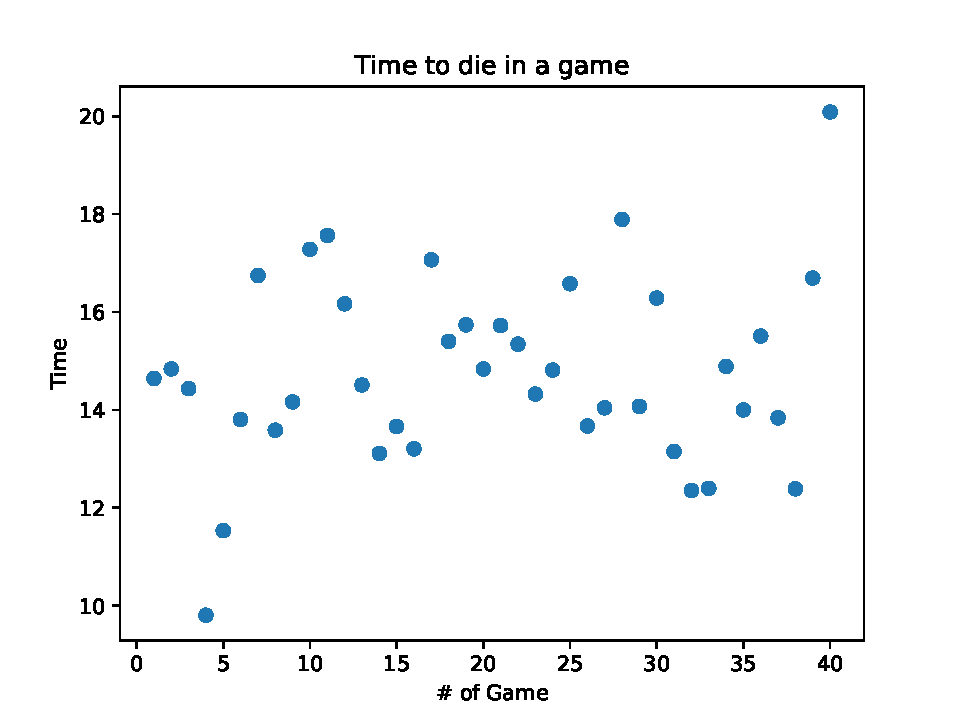
\includegraphics[scale=.7]{exerc/3.pdf}
    \caption{Primera parte.}
  \end{figure}
  \begin{figure}[H]
    \centering
    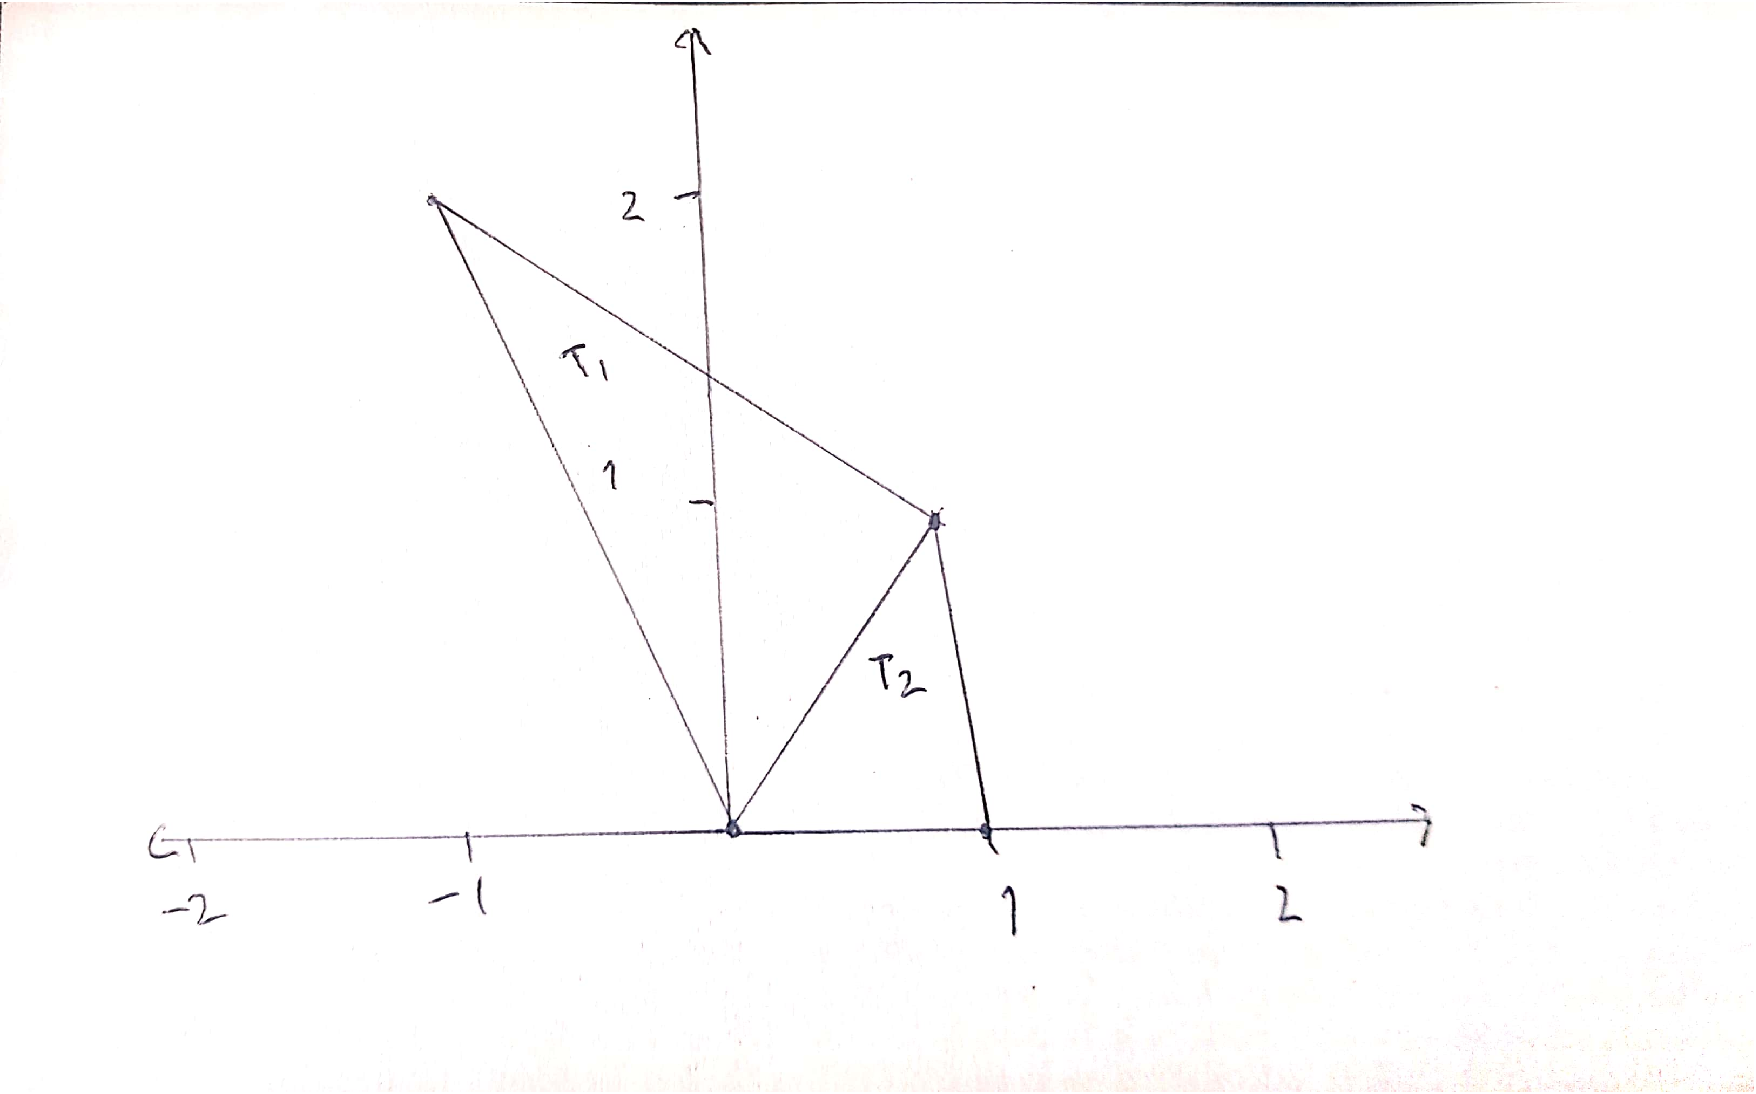
\includegraphics[scale=.7]{exerc/32}
    \caption{Segunda parte.}
  \end{figure}

    \begin{figure}[H]
    \centering
    \includegraphics[scale=.7]{exerc/33}
    \caption{Tercera parte.}
  \end{figure}

\item Los supuestos son:
  \begin{itemize}
  \item La dinámica de precios del activo está dada por un movimiento
    browniano geométrico, el precio es lognormal.
  \item El rendimiento medio esperado y la volatilidad del precio se
    mantien constante a través del tiempo.
  \item No existen costos de transacción.
  \item Todos los activos son perfectamente divisibles.
  \item No existen dividendos durante la vida de la opción.
  \item No existen oportunidades de arbitraje.
  \item Todos los agentes comparten exactamente la misma información,
    es decir, la información es simétrica.
  \item El activo puede negociarse de manera continua.
  \end{itemize}

  Y los enfoques metodológicos son:
  \begin{itemize}
  \item Se tiene un activo subyacente modelado por una ecuación
    diferencial estocástica.
  \item Se supone que el precio de una opción call $f$, sobre $S_t$ es
    de la forma $f = f(t, S_t)$.
  \item Se aplica la fórmula de Itô y se remplaza el diferencial por
    la EDE inicial.
  \item Discretizar la EDE original y la EDE obtenida de $f$.
  \item Se construye un portafolio, notado por $\pi$, tal que el
    tenedor tenga posición corta en el derivado y larga en una
    cantidad $\frac{\partial f}{\partial S_t}$ del activo:
    \begin{equation*}
      \pi = - f + S_t\frac{\partial f}{\partial S_t}
    \end{equation*}
  \item Discretizar la anterior ecuación y remplazar cada uno los
    términos.
  \item Ya que el portafolio es libre de riesgo, suponer que:
    $\Delta\pi =\pi r \Delta t$, con $r$ siendo la tasa de interés.
  \item Por último, remplazar las ecuaciones obteniendo una ecuación
    para $rf(t, S_t)$.
  \end{itemize}
\end{enumerate}
\end{document}
